\section{Motivation}

More and more people consume media from client-server based sources (e.g., Facebook, Netflix, Spotify, etc.) instead of traditional one-to-many sources (e.g., television, radio, etc.) that usually carry emergency alerts. The current solution to alerting users of client-server systems is to provide an emergency alert feed that websites and providers can periodically poll and then push to users. While television and radio broadcasters (and providers) are legally required to disseminate these messages, websites and ISPs\footnote{Companies that provide both (like AT\&T), only are required to send via the mandated medium} are not.\cite{cfr47}

More importantly, the existing systems treat the internet as a reliable black box, ignoring the increasing frequency and strength of cyber-attacks. In `traditional' emergency scenarios the internet is either present or not; physical cables are down or up. However, in a denial of service attack, the physical infrastructure is intact, but the ability for useful communication is heavily degraded. In a scenario where either terrorist or state actors decide to attack in both the physical \textit{and} cyber realms, citizens still need to be able to receive these critical alerts.

\section{Background}
\subsection{Trotsky}
The foundation for this project is Trotsky, a clean-slate internet framework that separates intra (L3) and inter (L3.5) domain abstractions, and allows for a proliferation of specialized network architectures. The forwarding appliance in Trotsky is the Trotsky Processor (TP): an end-point for an L3.5 pipe that forwards based on the L3.5 protocol agent of the incoming packet. New inter-domain architectures can be developed and deployed by simply adding a routing agent to TPs. In addition, new intra-domain architectures can be created and replaced within a domain without affecting the L3.5 architecture.

We leverage Trotsky both as a way of deployment and as a rationale for our design. Deployment in Trotsky is as simple as pushing a software update to TPs. We also use the L3.5 abstraction of domain-to-domain communication to simplify the problem from sending a message to every end-host to sending a message to every ISP. We aim to solve one specific problem: \textit{emergency} broadcast---with Trotsky this is allowed and even encouraged. There is no reason to add complexity to existing architectures or create a new all-encompassing architecture because Trotsky allows for an ecosystem of specialized architectures. 

\subsection{Existing Infrastructure}\label{infrabckgrnd}
The US public alert system has been around for over a half century\footnote{This paper focuses on the US, but most countries (if they have such systems) have similar designs.}. The system begins with FEMA initiating an alert and sending it to Primary Entry Points (PEPs) across the country via robust RF communication. PEPs are hardened sites that help spread the alert to local radio and TV stations (and can also serve as origin points for local alerts). FEMA (at the same time as the aforementioned broadcast) publishes alerts to an online information feed. All cellular providers and, as seen in a 2018 test of the system, a majority of radio \& television providers use this online feed. Ultimately, the FEMA message first goes to distributors, which then, in turn, deliver the alert to individual citizens. \cite{ipaws101}

The 2018 system test showed some interesting results about the effectiveness of the system. Overall only about 80\% of people received the alert, showing that there is room for improvement. Furthermore, most people that were surveyed received the alert on their smartphone, rather than radio or television (combined less than 10\% of respondents ). The cellular transmission caused a variety of issues, ranging from ensuing service outages, to receipt of dozens of duplicate alerts.\cite{weatest,everbridge}

\section{Design Overview}
Our design combines the abstractions provided by Trotsky with the hierarchical broadcast design provided by the current emergency broadcast infrastructure. Concretely, this means flooding an alert on L3.5, and then having ISPs push the message directly to citizens. 

\begin{figure}[tp]
\centering
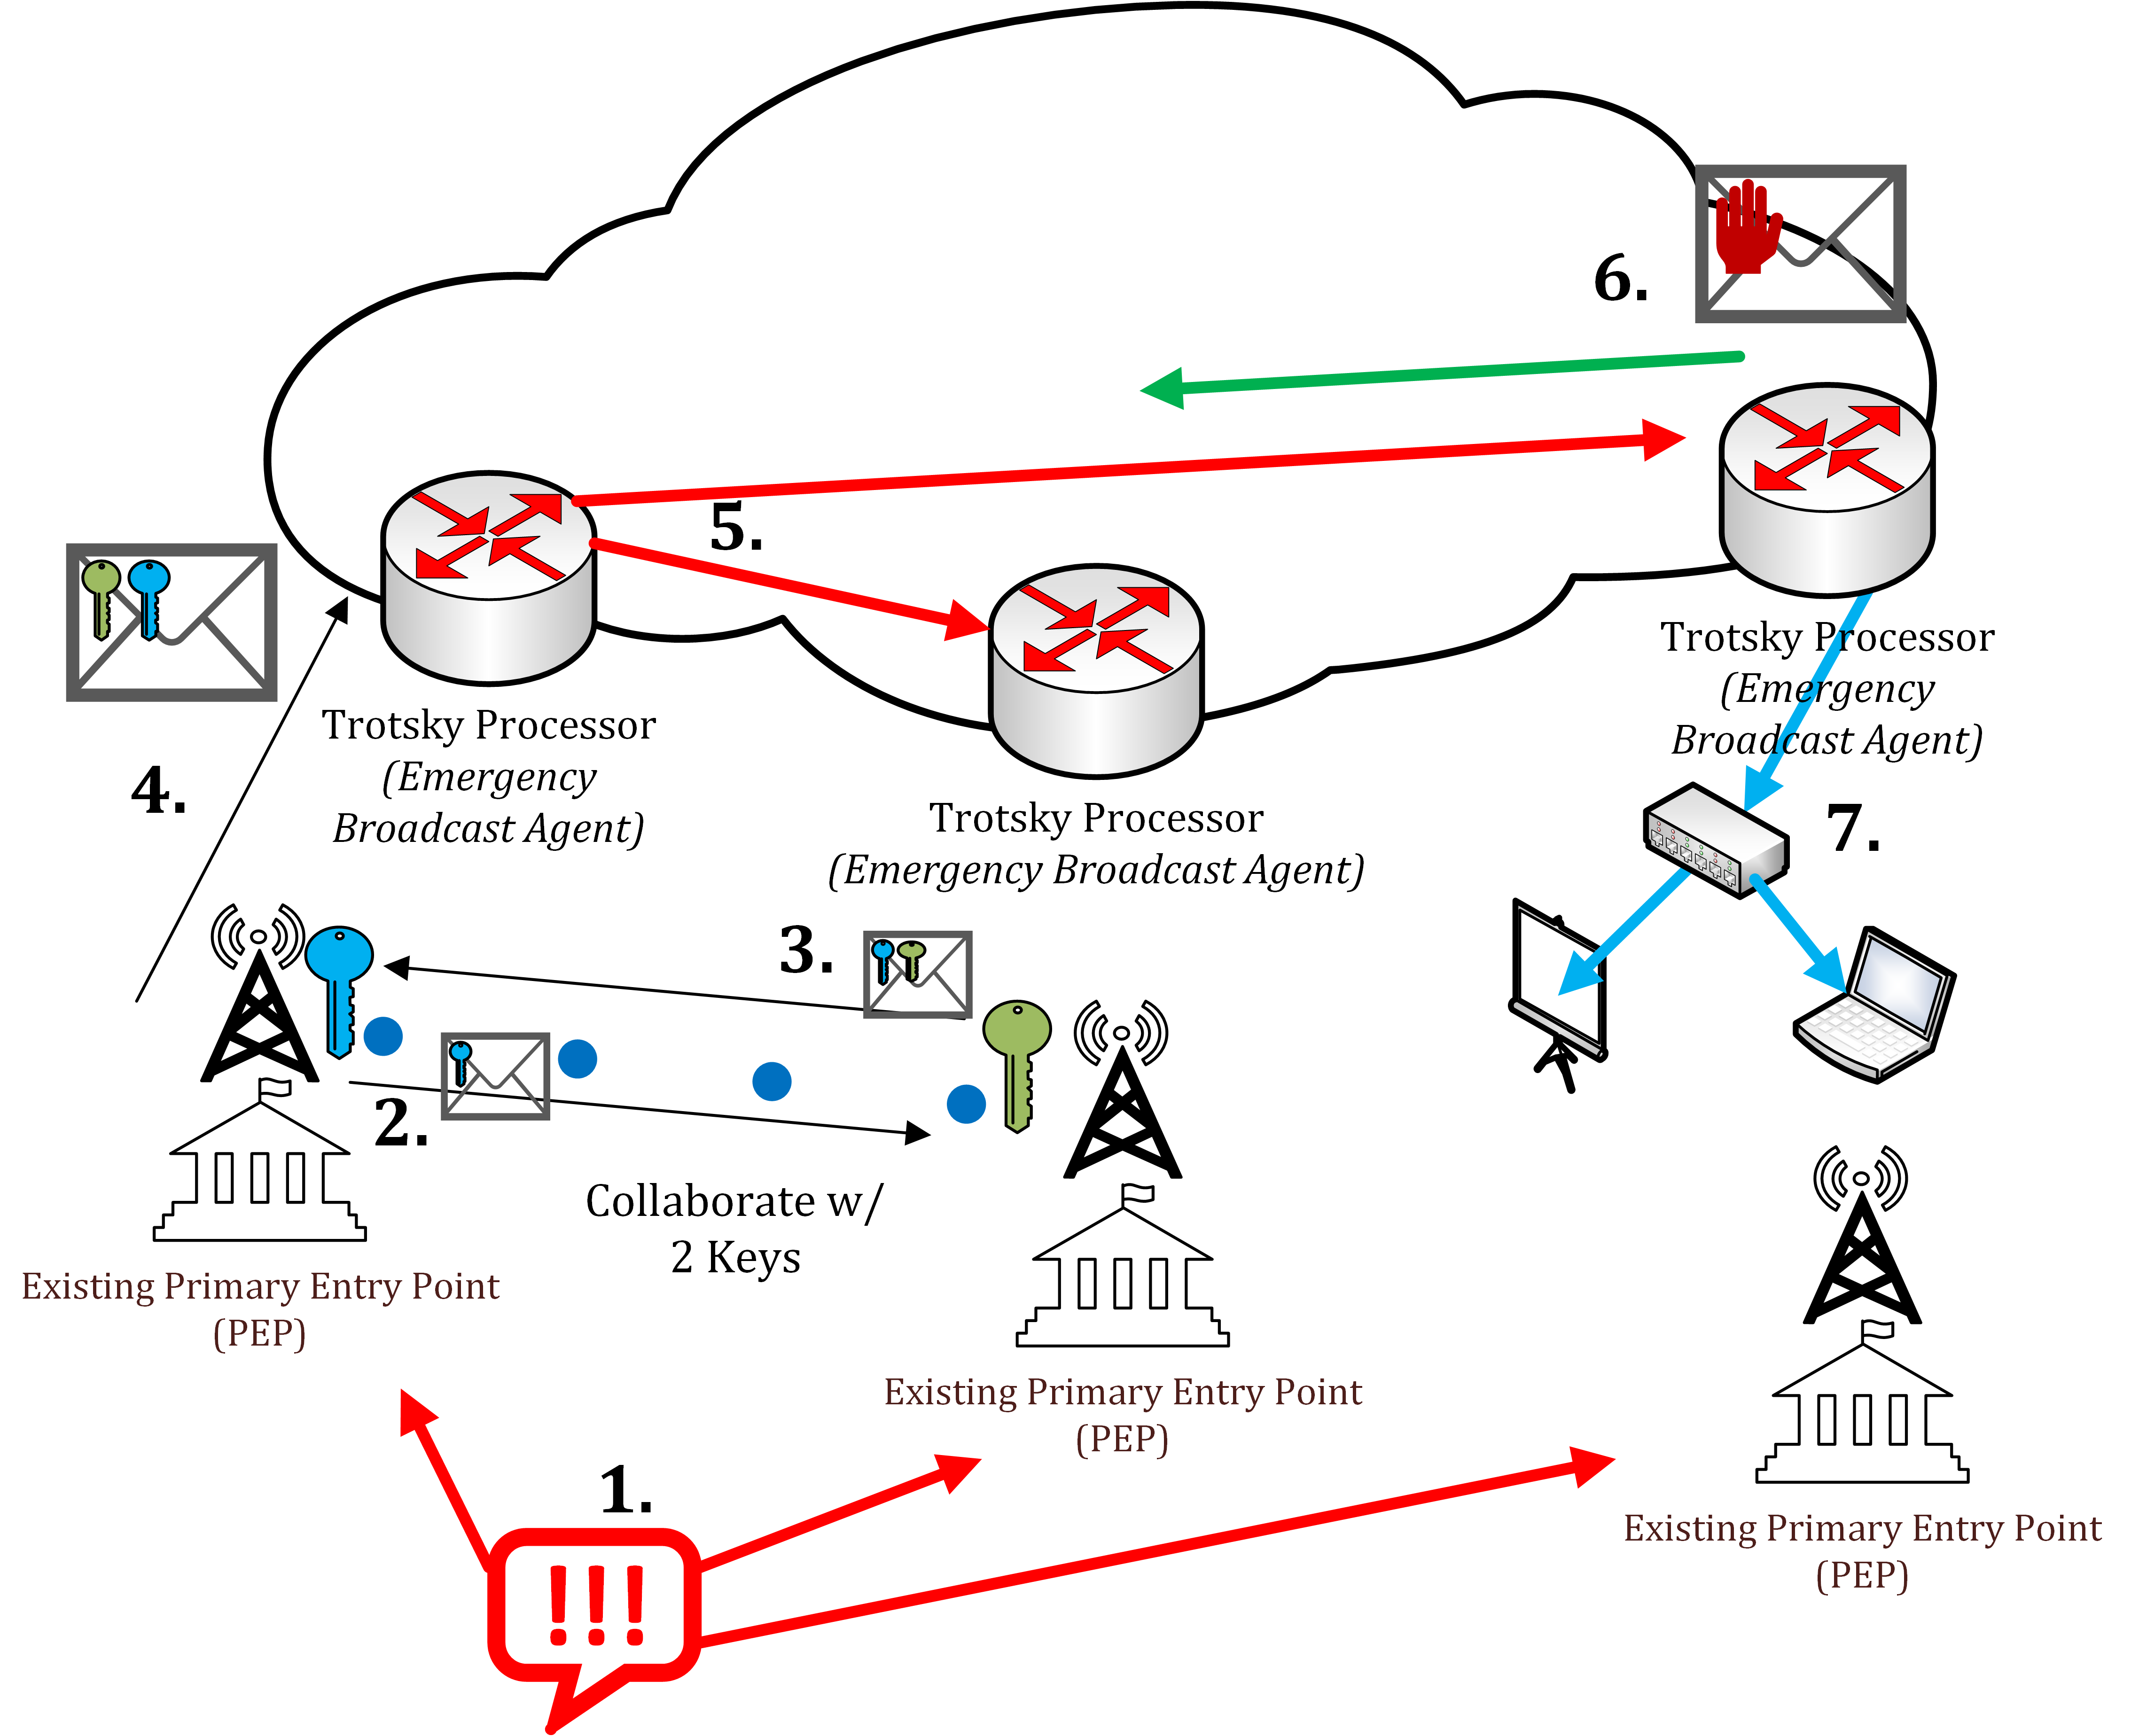
\includegraphics[width=8.5cm]{figures/full_diagram_v2.png}
\caption{Step-by-step process of a nation-wide broadcast}
\label{fig:brdcast}
\end{figure}


\subsection{Detailed Proposed Process}
The steps for a national alert solution using our proposed architecture are shown in Figure \ref{fig:brdcast}, and are described in detail below.

\textbf{1.} Some approved entity sends an out-of-band signed message to the PEPs\footnote{These are the same PEPs mentioned in section \ref{infrabckgrnd}} across the country. This step helps ensure that the message is inserted into multiple points of the internet, reducing the impact of network partition. 

\textbf{2. \& 3.} PEPs confer with each other (out-of-band) to reduce the risk of a compromised PEP (described in section \ref{acl}). 

\textbf{4.} PEPs then send the message to their ISP where the first TP receives the message. The TP ensures that the message has the correct signature (described in section \ref{acl}), dropping the message if it does not.

\textbf{5.} The TP initiates L3.5 flooding\footnote{Continual broadcast to all neighbors.} of the packetized message, encoding the data using a fountain code (described in section \ref{reliable}). Every TP that receives a packet from the message \textit{also checks} the signature before forwarding. If the signature does not match, the packet is dropped.

\textbf{6.} Each TP floods until its neighbor responds with `Message Received.' 

\textbf{7.} When each TP is able to decode the message, the owner of the TP (an ISP) will begin internal, intra-domain broadcast to its customers.

\\
Once messages get to an ISP, the ISP is responsible for the `last-mile' delivery to people. This delivery service can differ domain to domain. For a wireless provider, they may use the same SMS-based emergency alert system that is in use today. ISPs can use multicast, existing modem communication systems, or whatever technologies they may have. Finally, the host-based delivery is as simple as having browsers or OS vendors accepting special, verified `alert' packets. 

A local emergency broadcast would follow a similar procedure, but still differs in two main ways. First, it may not require cross validation with other PEPs. This is because a locality may only have one PEP, and an initiating authority would go directly to that PEP for broadcasting. Second, when the message is flooded on L3.5, TPs in different localities would not continue the broadcast\footnote{If a TP knew its neighbors were in the same location as the broadcast, it would forward the packets.}. 

To draw our discussion of the overall design to a close, we will now discuss how the packet layout enables the functionality of our architecture. The fields in the packet are shown in Figure \ref{fig:pckt}; everything `inside' of the L3.5 header was created as part of our proposal. The L3.5 header specifies that the TP should pass the packet to the Emergency Broadcast processing agent. The\textit{ Broadcast ID} is a flow number to differentiate between messages. The \textit{Total Number Sent} specifies how many packets the TP should receive before sending `Message Received.' This number will be larger than the number of packets needed for decoding the message and will be described in section \ref{reliable}. \textit{Location} specifies what region\footnote{Any standardized location format works (e.g., ZIP code, city, etc.)} the message is for, enabling local broadcast. The \textit{Crypto Signature} is integral to the verifying that the packet came from an authorized origin and has not been tampered. The \textit{Time Stamp} states when the message was initially sent. Together these two fields prevent replay-based attacks (messages with a valid signature and a stale time stamp will be dropped).
\begin{figure}[tp]
\centering
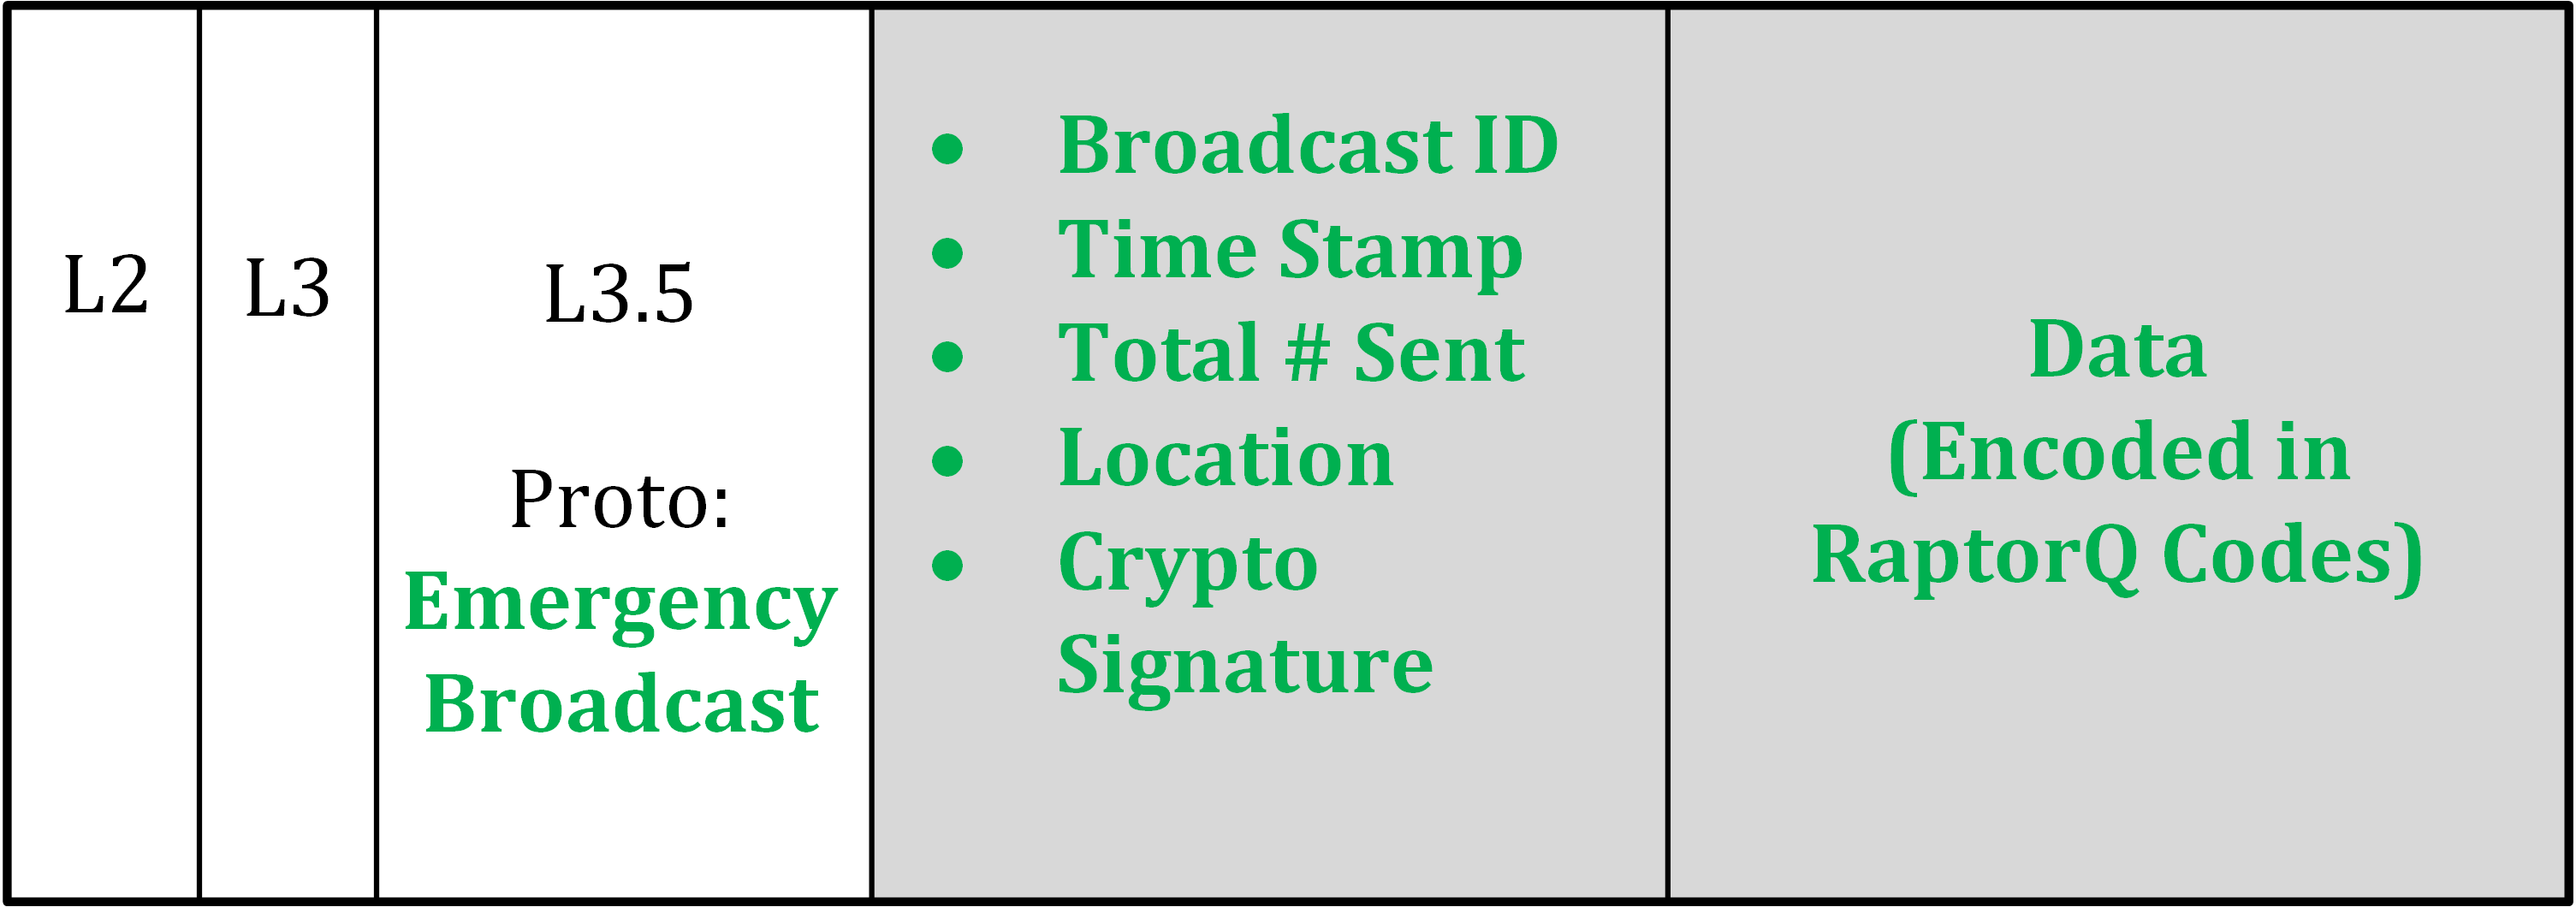
\includegraphics[width=8.5cm]{figures/packet_header_final.png}
\caption{Packet layout}
\label{fig:pckt}
\end{figure}

\subsection{Rationale}
The goal for this architecture is two-fold: \textbf{1)} robust message delivery and \textbf{2)} access control. We further worked with several key assumptions:  \textbf{A)} emergency broadcasts are relatively infrequent, \textbf{B)} Trotsky is the standard framework, and \textbf{C)} some central authority that must be trusted\footnote{This is meant in both having some sort of centralized key storage and also in the sense of having someone with absolute ability to launch an alert (the president)}. This prioritization led to the design we have here.  

Goal \textbf{1} and assumptions \textbf{B} allowed us to consider in-network solutions. End-to-end arguments over many lossy links\footnote{While the internet is usually \textit{not} lossy, in congestion-attack scenarios that we are concerned with, packet loss is common.} are weak because the per-link drop-probabilities are compounded and result in low chance of delivery. Trotsky allows us to place functionality in the network, reducing the number of links between logical endpoints, increasing robustness. In-network support also allows for extensions like increasing QoS levels for these alerts\footnote{To reiterate: this is an extension.}. 

Goal \textbf{1} and assumption \textbf{A} led us to the idea of flooding. This architecture is used for infrequent and \textit{urgent} events, meaning that degradation of other traffic is tolerable. Using BGP (or any `normal' inter-domain routing) paths increase the probability of message failure if links go down or are unstable; it also introduces unnecessary complexity. The use of many PEPs to introduce the message to the system also reduces the single-point-of-failure of having a truly centralized network entry point.

In the following section, we will focus on goal \textbf{2} and assumption \textbf{C}. 

\section{Access Control}\label{acl}
The goal of access control in our design is to protect users from false broadcasts and to ensure that they receive critical information in times of emergency. We limit the ability to broadcast messages on the network to a small group of trusted parties such as local and federal governments. Our network architecture is responsible for preventing malicious users from disseminating misinformation or spamming the network and its users with their messages.
\subsection{Overview}
To ensure that only authorized users can broadcast emergency messages on the network, we need to be able to verify the identity of the sender. We use a public key infrastructure, such as X.509 certificates\cite{x509}, to authenticate the identity of the sender. The federal government will act as the root certificate authority, which signs a root certificate to be stored in the trust store of every TP's Emergency Broadcast agent. The federal government is responsible for signing certificates for local governments to act as intermediate certificate authorities. Both the root certificate authority and intermediate certificate authorities are able to sign end entity certificates for members of their organization to use to send messages through the network.
\subsection{Signing/Verifying Process}
In order to send a message using the Emergency Broadcast Architecture, the sender first encodes the message using fountain codes (described in section \ref{reliable}) and signs the encoded message along with the packet header. The signature and chain of certificates are included in the packet's header and the encoded message is sent in the body of the packet. 

To verify the validity of a packet at a TP, the chain of certificates is first validated by making sure the end entity certificate is signed by a valid intermediate certificate or the root certificate, and if there is an intermediate certificate it must be signed by the root certificate. Next, the location field is enforced by checking that the intermediate certificate belongs to the correct local authority specified in the location field of the header. If packet is part of a national broadcast, then the end entity certificate must be signed directly by the root certificate. Finally, the signature of the packet and timestamp are checked to make sure that the packet has not been tampered with and that it was sent recently to prevent replay attacks.
\subsection{Threat Model}
In our architecture, we trust that the government, both local and federal is not malicious.  Network operators, and hardware vendors can be singularly malicious as their impact would only affect their local domain (a national alert would not happen). We assume that network operators and hardware vendors are not collectively malicious. The main threats we protect against are other users of the internet. Since anyone is able to send a packet that uses the Emergency Broadcast L3.5 header, we must prevent malicious users of the internet from trying to broadcast their own message to all the other users of the internet. We also need to make sure that the legitimate messages that get sent are actually correct and received by every user. This is why our architecture provides authenticity, integrity, and reliability.
By using certificates and having the sender sign both the message and the timestamp, we ensure the authenticity and integrity of the message and prevent replays of the same message. With Trotsky, we are able to provide reliability as part of the network and we further improve reliability through encoding the message with RaptorQ fountain codes which we describe in section \ref{reliable}.
\subsection{Extensions}
Security could be further improved upon at the application layer through private key management. One possible improvement is the sharing of private keys across multiple PEPs through secret sharing. With one private key split across multiple PEPs, it would require multiple PEPs to agree on a message in order to recover the private key required to sign the packet. By requiring the consensus of multiple PEPs to send a message, we protect against rogue PEPs from sending messages by themselves and from accidental message broadcasts. Another extension is to handle lost or stolen keys to prevent malicious use of the stolen keys. We can achieve this through the use of certificate revocation lists(CRL) to invalidate existing signed certificates before their expiration in the case that the private key associated with the certificate is compromised. Every TP could periodically poll and store this list locally and not accept any messages that are signed with an invalidated certificate.


\section{Reliable Transmission}\label{reliable}
In order to increase the speed and reliability of message transmission, we will use RaptorQ fountain codes. We will use RaptorQ and rateless codes interchangeably throughout this paper. The idea of fountain codes is that a finite source of $k$ symbols can be transformed into an arbitrarily long stream of non-redundant symbols. Furthermore, the receiver only needs to receive \textbf{any} $k + \epsilon$ symbols to recover the original message. For RaptorQ, $\epsilon = 0$ and $\epsilon = 2$ give, respectively, a $99\%$ and $99.9999\%$ chance of recovery.\cite{raptorq, raptorqpresent}

RaptorQ encoding also provides high performance through linear time encoding and decoding, reducing the burden on TPs\footnote{Specifically that the encoding/decoding scheme does not rely on specialized hardware}. Codornices, a RaptorQ package from ICSI, recently released performance results. For a 128 kB message on x86, the encode and decode took under $0.5$ ms each, and was able to produce/consume at a rate of $2$ Gbps\cite{raptorqperf}. This performance is definitely sufficient for our application, as will be described in the following section.

\subsection{Use in our system}
In our design we encode a message once; it is only encoded when it arrives at the first TP. All subsequent TPs (in other domains) decode the message (for intra-domain broadcast) and resend the \textit{already encoded} message to neighbors. Since we are reducing a potentially infinite stream to a finite length, we must ensure that nodes receive \textit{more} packets than are needed to only reconstruct the message. For a message of $k$ blocks, we set the \textit{Total Number Sent} packet field (refer to Figure \ref{fig:pckt}) to $k\cdot f_{overshoot}$. This overshoot value is not permanently fixed and can be tuned: a large $f_{overshoot}$ uses more bandwidth, but ensures more packets for future nodes to re-transmit, while a small $f_{overshoot}$ (specifically $1$) is just blind sending of a message.

The choice to not use full RaptorQ decoding and encoding capabilities at each step was based on the concern of blocking\footnote{`Blocking' was chosen over `store-and-forward' in order to emphasize that this is on a per \textbf{message} basis}, or waiting for an entire message to arrive before flooding. All the time that one node spends waiting to receive the remainder of a message is time wasted in transmission. This is further explored in the evaluation.

\section{Evaluation}
For our evaluation we used the python networkx library to model the high level behavior of different propagation modes.\cite{nwx}
For network topologies, we used an abridged Rocketfuel ISP level map. \cite{rocketfuel}

\begin{figure}[tp]
\centering
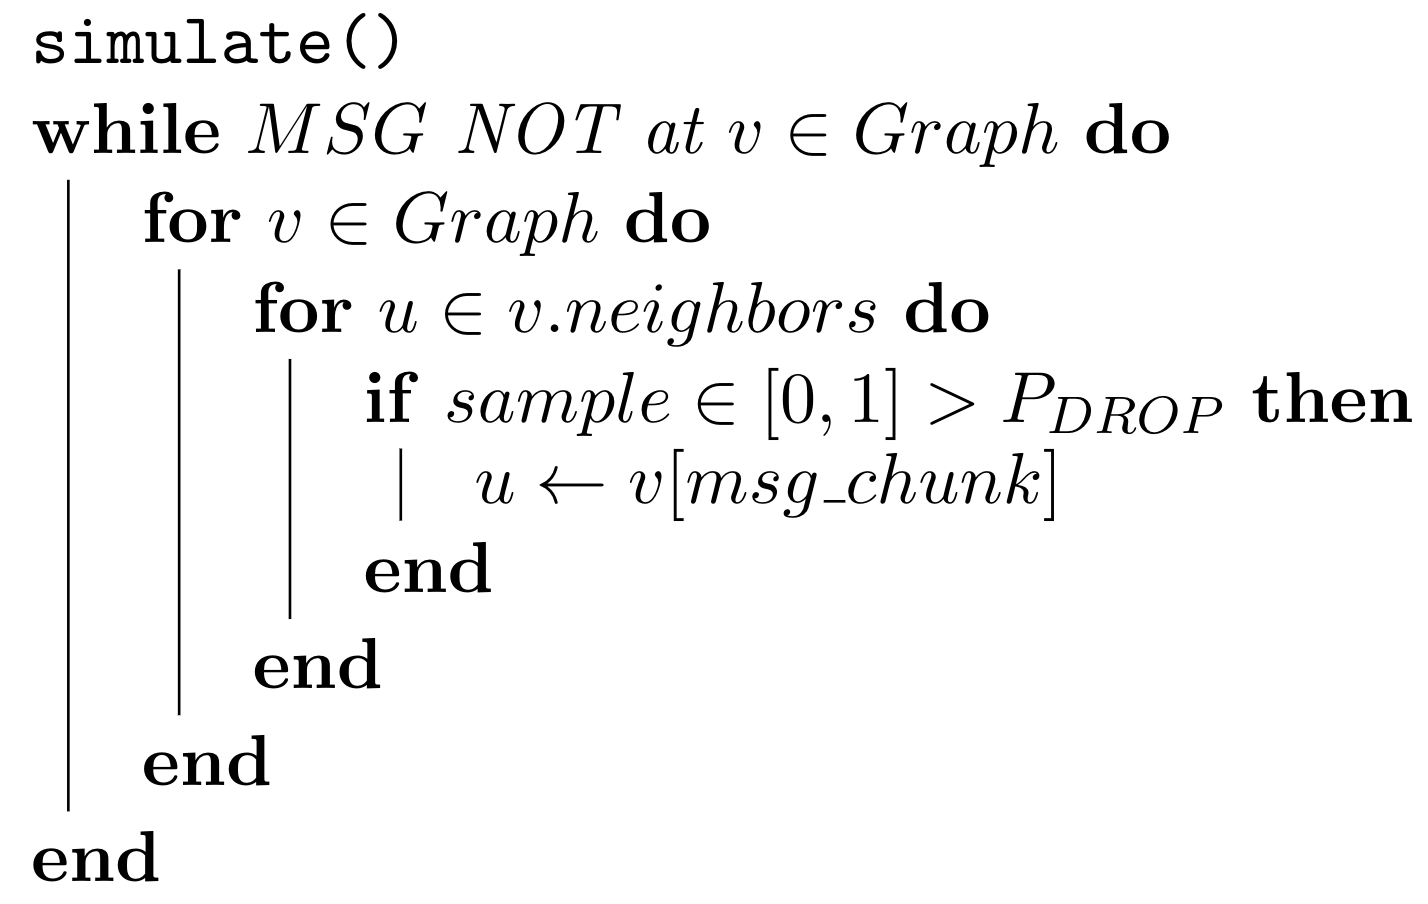
\includegraphics[width=6cm]{figures/algo_v2.png}
\caption{Basic simulation algorithm used}
\label{algo:a1}
\end{figure}

\subsection{Simulation Design}
The simulator provides a step-based simulation of propagation of packets until all nodes have received the full message. The pseudocode is provided in Figure \ref{algo:a1}. The simulator makes sure that this abstraction of lock-step propagation is maintained. For example, when on iteration $i$, and node $u$ sends $p_{a+1}$ to $v$, when $v$ gets its turn to send on iteration $i$, it \textbf{cannot} send $p_{a+1}$. The simulation stops when all nodes have received the message (this metric differs per sending method). 

We modeled ACK-based senders, rateless senders (decode-only), and blocking rateless senders (encode and decode at each step). To simulate ACK-based sending, each node keeps track of the largest `sequence number` that each neighbor has received. Nodes repeatedly send one packet until the neighbor explicitly tells it to move on. 

For rateless senders, each node sequentially goes through received packets and blindly sends them (there is no knowledge if the receiver has received it). The first node is given $len(MSG)\cdot f_{overshoot}$ packets to begin sending. The simulation ends when all nodes have received any set of $len(MSG)$ distinct packets. The blocking rateless sender cannot transmit until it has received $len(MSG)$ packets, but, unlike the rateless one, it sends an infinite stream of packets until the simulation ends.

\subsection{Experimental Setup}
For each experiment we defined a link-based drop probability value, selected a given propagation method and ran the simulation. For each set of control variables we repeated the simulation 100 times to get a strong sample size. For all experiments, we selected one sender node (at random from the graph) and sent a 15-packet-long message. Unless otherwise specified, the rateless sender uses a $f_{overshoot}$ of $2$.

We were only concerned with relative performance of methods, not absolute performance. Drops were used to model congestion because routing devices under attack would begin dropping packets once buffers filled up. We measured performance in terms of "Numbers of Iterations," or the amount of time the simulation ran for. Converting from this to actual propagation time would look something along the lines of $Num\_of\_Iterations\cdot \frac{\overline{Transmission\_Latency}}{\overline{Link\_Bandwidth}}$\footnote{We do not intend to treat these as any form of real world estimations, and this equation is just a hypothetical in the right direction}.

\subsection{Results}

\begin{figure}[tp]
\centering
\noindent
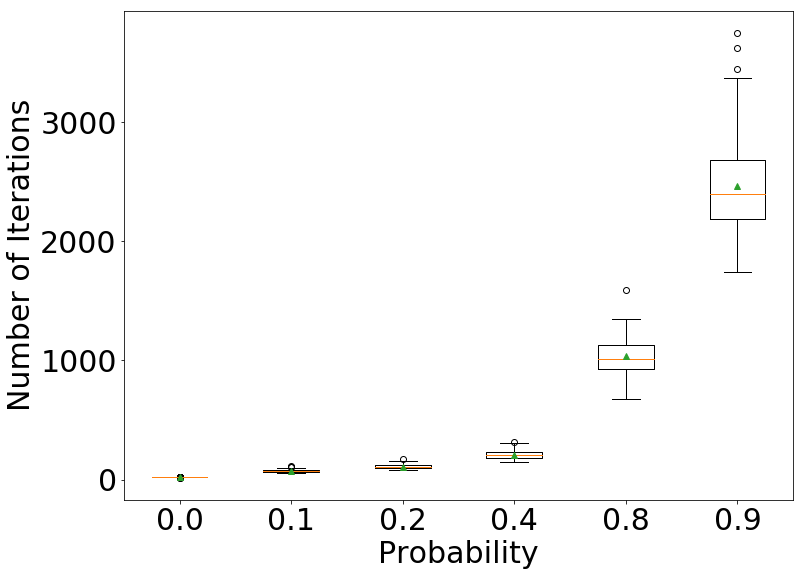
\includegraphics[width=8cm]{figures/ACK_FINAL.png}
\caption{Box-and-Whisker plot of the ACKing sender }
\label{graph:ack}
\end{figure}

\begin{figure}[tp]
\centering
\noindent
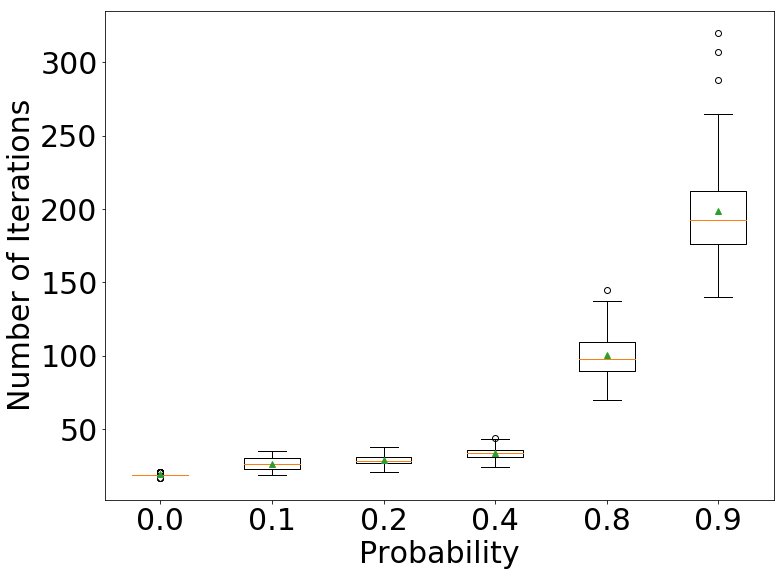
\includegraphics[width=8cm]{figures/rateless_FINAL.png}
\caption{Box-and-Whisker plot of the rateless sender}
\label{graph:rateless}
\end{figure}


Our results are summarized in Figures \ref{graph:ack}, \ref{graph:rateless}, \ref{graph:ackvsrateless}, \ref{graph:ackvsratelessLOG}, \ref{graph:blockingvsnot}, and \ref{graph:varyParams} \footnote{Note that the drop probability of $0.99$ was excluded from Figure \ref{graph:ack} and Figure \ref{graph:rateless} in order to increase readability.}.

The first two graphs show the performance of the ACK-based sender (Figure \ref{graph:ack})and rateless sender (Figure \ref{graph:rateless}) relative to themselves as the probability of packet-loss increases. From these graphs, we can see how the message propagation time would vary based on the severity of packet loss. These graphs provide a stand-alone baseline for each major sending method. It should be noted that y-axis on these graphs are \textbf{10x} greater in Figure \ref{graph:ack} as compared to Figure \ref{graph:rateless}.

Figure \ref{graph:ackvsrateless} compares the average performance of the ACK-based sender and the rateless sender as drop probability increases. The main takeaway from this graph is that the performance of ACK-based sending rapidly degrades when the drop probability approaches $100\%$. To better understand the difference between these two senders at lower drop probabilities, refer to Figure \ref{graph:ackvsratelessLOG}, which uses a logarithmic $y$-axis. Even for mild conditions, the rateless sender is almost \textbf{10x} faster. 

The remaining graphs focus on comparisons between rateless senders. Figure \ref{graph:blockingvsnot} shows a direct comparison of the blocking rateless and 'normal' rateless senders. Both senders have relatively similar performance throughout all drop probability scenarios. The difference at the high drop probability is more pronounced for the blocking rateless sender, but is only ~1.5x bigger than the rateless sender. Returning to Figure \ref{graph:ackvsratelessLOG}, it reveals that these two sending methods are at a roughly constant separation of roughly 2x.

Figure \ref{graph:varyParams} compares the baseline rateless sending (which uses $f_{overshoot}$ $=$ $2$) , with $f_{overshoot} = 4$ and $f_{overshoot} = 8$. This figure is the \% difference of the ratio of Number of Iterations on higher factors as compared with the baseline. All values represented here are less than 1.1x different. This shows that while increasing the overshoot factor improves performance, the result is small.

The clearest result is not surprising: rateless sending outperforms ACK-based sending. This makes sense because an ACK-based sender needs to traverse each link \textit{twice} for any given packet. 

The results between rateless senders are more surprising. The blocking, rateless sender performed relatively well, staying within a roughly constant factor of the non-blocking version. The impact of waiting to send (especially for high drop rates) seems to be countered by the infinite stream. With regards to the standard rateless sender, the choice of $f_{overshoot}$ does not seem to matter much beyond a factor of $2$. The increase of $f_{overshoot}$ to $4$ and $8$ resulted in materially similar results.

\begin{figure}[tp]
\centering
\noindent
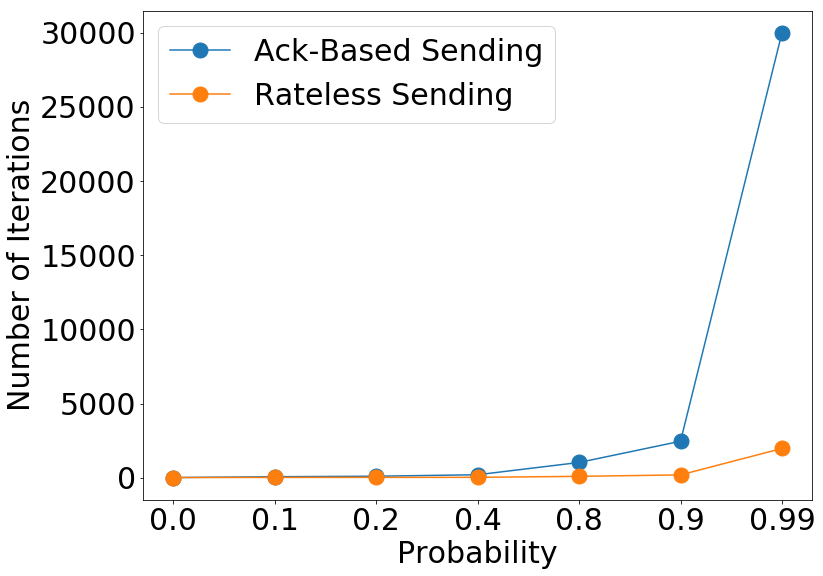
\includegraphics[width=8cm]{figures/ACK_RATELESS_FINAL.png}
\caption{Comparison of the ACKing and rateless senders}
\label{graph:ackvsrateless}
\end{figure}

\begin{figure}[tp]
\centering
\noindent
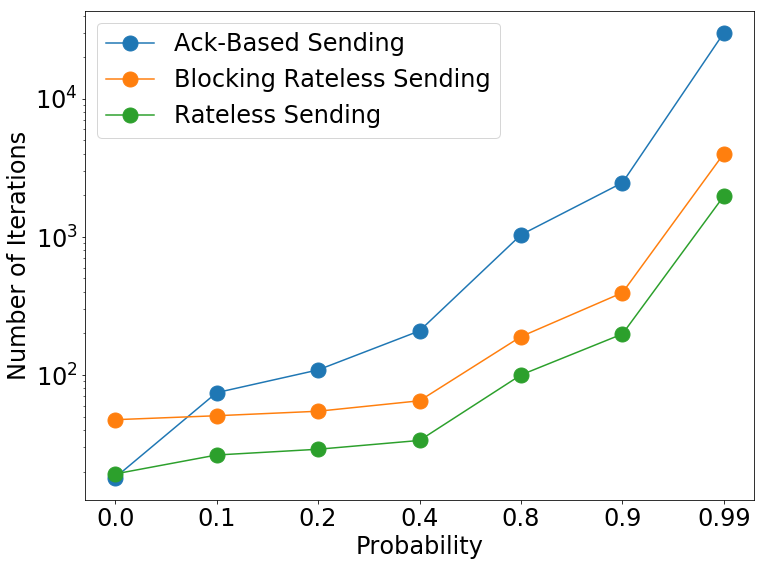
\includegraphics[width=8cm]{figures/TRIPLE_FINAL.png}
\caption{Comparison of the ACKing and two rateless senders on a log y-axis}
\label{graph:ackvsratelessLOG}
\end{figure}

\begin{figure}[tp]
\centering
\noindent
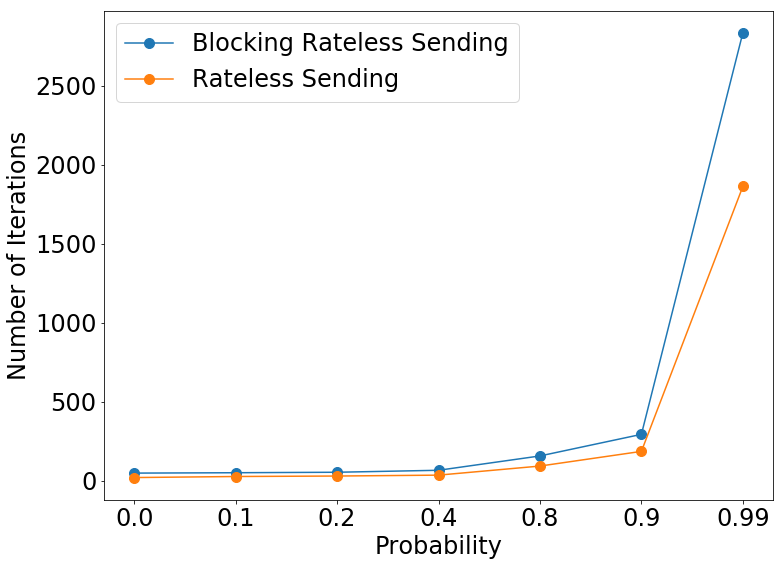
\includegraphics[width=8cm]{figures/big_font/BLOCKING_RATELESS_BETTER.png}
\caption{Comparison of the blocking and non-blocking rateless senders}
\label{graph:blockingvsnot}
\end{figure}

\begin{figure}[tp]
\centering
\noindent
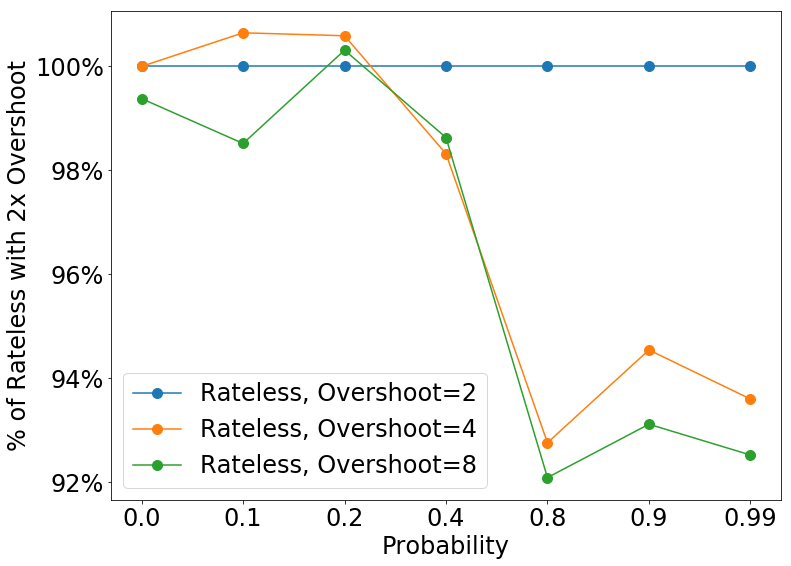
\includegraphics[width=8cm]{figures/FACTOR_VARY_FOCUS.png}
\caption{Comparison of a Rateless senders with various overshoot factors}
\label{graph:varyParams}
\end{figure}

\section{Conclusion}
In this paper we presented a new Emergency Broadcast Architecture that interleaves existing infrastructure with a flexible internet framework to produce a simple, robust design. We achieved our goal of reliability through RaptorQ encoding on a hop-to-hop basis and our goal of access control by leveraging  public key cryptography and existing PEPs. Overall, our design meets the needs of a future-proof emergency alert system. With our assumption of working in a "Trotksy World," we leave open paths for future research into merging our designs in the existing emergency alert and internet infrastructure to increase the robustness of the national broadcast system.

\textbf{Acknowledgements:} We thank Murphy McCauley for helping us get started with this idea. We also are grateful for Nick Weaver, who helped us solidify our security model.

